\documentclass{beamer}

\usepackage{Haust2017glærur}

\author{Eiríkur Ernir Þorsteinsson}

\title{Tölvunarfræði 1a}
\subtitle{Vika 5, fyrri fyrirlestur}

\begin{document}

\begin{frame}
\titlepage
\end{frame}

\section{Inngangur}

\begin{frame}{Í síðasta þætti\ldots}
\begin{itemize}
 \item \texttt{for} lykkjur
 \begin{itemize}
  \item Áhyggjuefni við að stækka vigra
 \end{itemize}
 \item Hreiðraðar \texttt{for} lykkjur
\end{itemize}
Kaflar: 5.1, 5.2
\end{frame}

\begin{frame}{Upprifjun}
\vspace{\baselineskip}
\begin{columns}
\column{0.5\textwidth}
Skráin \texttt{forExample.m}
\begin{center}
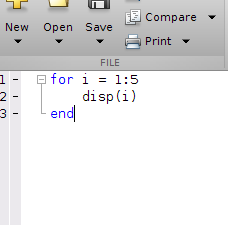
\includegraphics[width=0.8\linewidth]{Pics/for-example}
\end{center}
\column{0.5\textwidth}
Keyrsla í skipanaglugga
\begin{center}
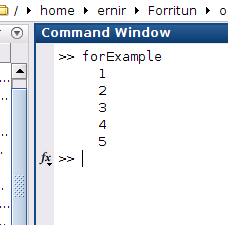
\includegraphics[width=0.8\linewidth]{Pics/for-example-run}
\end{center}
\end{columns}
\end{frame}

\section{while lykkjur (5.3)}

\begin{frame}{while-lykkjur}
\begin{itemize}
 \item Auk talningalykkjunnar \texttt{for} höfum við líka skilyrta lykkju í \texttt{Matlab}
 \begin{itemize}
  \item Sú lykkja kallast \texttt{while}
  \item Setningar lykkjunnar eru endurteknar á meðan tiltekið skilyrði er satt
  \item Vitum ekki endilega fyrirfram hversu oft lykkjan er ítruð
  \item Þetta gæti jafnvel verið endalaus lykkja (e. \emph{infinite loop})\footnote{Verðum þá að hætta með Ctrl-C}
 \end{itemize}
\end{itemize}
\end{frame}

\begin{frame}[fragile]{while-lykkjur}
\begin{itemize}
 \item Almennt form \texttt{while}-lykkja:
\begin{verbatim}
while skilyrði
  skipanir
end
\end{verbatim}
\pause
 \item Fyrst er skilyrðið reiknað
 \begin{itemize}
  \item Ef gildi þess er satt þá eru skipanirnar framkvæmdar (svipað og if-setning)
 \end{itemize}
 \item Eftir að keyrslu skipananna er lokið er skilyrðið reiknað aftur
 \begin{itemize}
  \item Sé skilyrðið aftur satt, þá eru skipanirnar keyrðar aftur
  \item Skipanir lykkjunnar þurfa að hafa áhrif á skilyrðið, annars höfum við endalausa lykkju
 \end{itemize}
\end{itemize}
\end{frame}

\begin{frame}[fragile]{Dæmi um while-lykkjur}
\begin{columns}
\column{0.5\textwidth}
\vspace{0.8cm}

Dæmi um lykkju:
\begin{minted}[frame=lines]{matlab}
rSum = 0;
while rSum < 100
   rSum = rSum + rand();
end
\end{minted}
Hér er \texttt{rSum} $0$ í upphafi, svo skilyrðið er satt. Breytan hækkar svo í hverri ítrun um tölu á opna bilinu $0$ til $1$, lykkjan hættir að lokum.\pause
\column{0.5\textwidth}
En hvað gerir lykkjan
\begin{minted}[frame=lines]{matlab}
rSum = 0;
while rSum < 100
   rSum = rSum - rand();
end
\end{minted}
?
\pause

Þetta er endalaus lykkja, skilyrðið verður aldrei ósatt.
\end{columns}
\end{frame}

\begin{frame}[fragile]{Keyra þar til notandi gerir rétt}
\begin{itemize}
 \item Viljum stundum biðja notanda um inntak endurtekið þar til viðkomandi slær inn rétt inntak
\end{itemize}
\begin{minted}[frame=lines]{matlab}
num = input('Sláið inn jákvæða tölu: ');
while num < 0
   disp('Ólöglegt gildi.');
   num = input('Sláið inn jákvæða tölu: ');
end
fprintf('Takk fyrir, talan er %.2f\n', num);
\end{minted}

\end{frame}


\begin{frame}[fragile]{Keyra þar til notandi segir annað}
\begin{minted}[frame=lines]{matlab}
% Lesa tölur frá notanda inn í vigur
% Lesið inn þar til notandi svarar 'n'

n = 0; v = [];
svar = 'j'; % a.m.k. ein tala lesin inn
while upper(svar) ~= 'N'
    n = n + 1;
    v(n) = input('Sláðu inn tölu: ');
    svar = input('Fleiri tölur (j/n)? ','s');
end
\end{minted}
\end{frame}

\subsection{Samanburður for og while}

\begin{frame}[fragile]{Hermun á for-lykkju}
\vspace{\baselineskip}
Hægt er að herma eftir for-lykkju með \texttt{while}
\begin{columns}
\column{0.5\textwidth}
\begin{minted}[frame=lines]{matlab}
for i = 1:n
  disp(i);
end
\end{minted}
\column{0.5\textwidth}
\begin{minted}[frame=lines]{matlab}
i = 1;
while i <= n
    disp(i);
    i = i + 1;
end
\end{minted}
\end{columns}
\begin{center}
jafngilt!
\end{center}
\end{frame}

\begin{frame}[fragile]{Hermun á for-lykkju}
\vspace{\baselineskip}
Örlítið erfiðara er að herma \texttt{for} lykkju sem vinnur yfir almennan vigur með \texttt{while}
\begin{columns}
\column{0.5\textwidth}
\begin{minted}[frame=lines]{matlab}
for i = [5 2 9 3]
    disp(i);
end
\end{minted}
\column{0.5\textwidth}
\begin{minted}[frame=lines]{matlab}
v = [5 2 9 3];
i = 1;
while i <= length(v)
    disp(v(i));
    i = i + 1;
end
\end{minted}
\end{columns}
\begin{center}
jafngilt!
\end{center}
\end{frame}

\subsection{break og continue}

\begin{frame}[fragile]{Að hætta í lykkju}
\vspace{\baselineskip}
\begin{itemize}
 \item Hægt er að ``hoppa út úr'' lykkju með lykilorðinu \texttt{break}
 \begin{itemize}
  \item Þá hættir lykkjan og skipanirnar sem koma á eftir \texttt{break} eru ekki framkvæmdar
 \end{itemize}
\end{itemize}
\begin{columns}
\column{0.3\textwidth} 
Almennt snið:
\column{0.7\textwidth}
\begin{verbatim}
while lykkjuskilyrði
   skipanir
   if skilyrði
      break
   end
   aðrar skipanir
end
\end{verbatim}
\end{columns}
\end{frame}

\begin{frame}[fragile]{Að fara áfram í lykkju}
\vspace{1.5\baselineskip}
\begin{itemize}
 \item Hægt er að hoppa yfir í næstu ítrun lykkju með lykilorðinu \texttt{continue}
 \begin{itemize}
  \item Þá hættir akkúrat sú ítrun lykkjunnar
  \item Farið beint í að athuga næsta skilyrði (í \texttt{while} lykkju) eða að keyra fyrir næsta stak í sviði (í \texttt{for})
 \end{itemize}
\end{itemize}
\begin{columns}
\column{0.3\textwidth} 
Almennt snið:
\column{0.7\textwidth}
\begin{verbatim}
while lykkjuskilyrði
   skipanir
   if skilyrði
      continue
   end
   aðrar skipanir
end
\end{verbatim}
\end{columns}
\end{frame}

\begin{frame}[fragile]{Tvær (undarlegar) lykkjur}
\vspace{\baselineskip}
Hversu oft keyra þessar lykkjur?
\begin{columns}
\column{0.5\textwidth}
\begin{minted}[frame=lines]{matlab}
x = 1;
while x >= 1
  disp(x)
  if x == 1
    break
  end
  x = x + 1;
end
\end{minted}
\column{0.5\textwidth}
\begin{minted}[frame=lines]{matlab}
x = 1;
while x <= 1
  disp(x)
  if x == 1
    continue
  end
  x = x + 1;
end
\end{minted}
\end{columns}
\pause Sú til vinstri keyrir einu sinni, sú til hægri er endalaus
\end{frame}


\begin{frame}[fragile]{Fyrirlestraræfing}
\begin{columns}
\column{0.6\textwidth}
\begin{enumerate}
    \item Hvert er gildi \texttt{y} í lok lykkjunnar hér til hliðar? ( Reynið að leysa án þess að slá inn)
    \item Skrifið \texttt{while}-lykkju sem er jafngild \texttt{for}-lykkjunni hér til hliðar
\end{enumerate}
\column{0.4\textwidth}
\begin{minted}[frame=lines]{matlab}
x = 0; y = 13;
while x < y
    x = x + 1;
    y = y - x;
end
\end{minted}
\begin{minted}[frame=lines]{matlab}
for i = 10:-1:1
    disp(i);
end
\end{minted}
\end{columns}
\end{frame}

\section{Vigurkóðun (5.4)}

\begin{frame}{Vigurkóðun}
\begin{itemize}
 \item Lykkjur eru mjög mikilvægar í flestum forritunarmálum
 \begin{itemize}
  \item \ldots líka í Matlab!
 \end{itemize}
 \item Í Matlab er þó oft hægt að komast hjá því að nota lykkjur
 \begin{itemize}
  \item Umritum kóða, sem notar lykkju, yfir í að nota sérstakar viguraðgerðir
  \item Þetta kallast vigurkóðun (e. \emph{vectorization})
  \item Vigurkóði er styttri og oftast hraðvirkari
 \end{itemize}
\end{itemize}
\end{frame}

\begin{frame}[fragile]{Reiknivirkjar á vigra og fylki}
\vspace{\baselineskip}
\begin{itemize}
 \item Þegar við viljum ``gera eitthvað'' við hvert stak fylkis er hægt að nota \texttt{for}-lykkju
 \item En oft er hægt að beita viguraðgerðum í staðinn
\end{itemize}
Dæmi: Margfalda öll stök vigurs með 3
\begin{columns}
\column{0.5\textwidth}
\begin{minted}[frame=lines]{matlab}
for i = 1:length(v)
    v(i) = v(i)*3;
end
\end{minted}
\column{0.5\textwidth}
\begin{minted}[frame=lines]{matlab}
v = v*3;
\end{minted}
\end{columns}
\begin{center}
 jafngilt!
\end{center}
\end{frame}

\begin{frame}[fragile]{Vigurkóðun}
\begin{columns}
\column{0.5\textwidth}
\begin{itemize}
 \item Þegar við sjáum vandamál sem er greinilega leysanlegt með lykkju ættum við að hugsa\ldots
 \begin{itemize}
  \item getum við notað viguraðgerðir?
  \item getum við notað föll sem virka á vigra?
 \end{itemize}
 \item Dæmi til hliðar: Fall sem finnur formerki talna í fylki
\end{itemize}
\column{0.5\textwidth}
(Bls. 176 í bók)
\begin{minted}[frame=lines, fontsize=\scriptsize]{matlab}
function outmat = signum(mat)
[r c] = size(mat);
for i = 1:r
    for j = 1:c
        if mat(i,j) > 0
            outmat(i,j) = 1;
        elseif mat(i,j) == 0
            outmat(i,j) = 0;
        else
            outmat(i,j) = -1;
        end
    end
end
end
\end{minted}
\end{columns}
\end{frame}

\begin{frame}[fragile]{Vigurkóðun}
\begin{columns}
\column{0.5\textwidth}
\begin{itemize}
 \item Svo vill til að Matlab er með innbyggt fall fyrir nákvæmlega þetta
 \begin{itemize}
  \item \ldots alltaf góð hugmynd að athuga hvort slíkt sé til
  \item Óþarfi að finna upp hjólið (nema í skólaverkefnum)
 \end{itemize}
\end{itemize}
\column{0.5\textwidth}
\begin{minted}[frame=lines]{matlab}
>> a = [0 4 -3; -1 0 2];
>> signum(a)
ans =
     0     1    -1
    -1     0     1
>> sign(a)
ans =
     0     1    -1
    -1     0     1
\end{minted}
\end{columns}
\end{frame}

\section{Tímamælingar (5.5)}

\begin{frame}{Tímamælingar í Matlab}
\begin{itemize}
 \item Við viljum oft mæla hversu langan tíma ýmsar skipanir taka 
 \item Til þess höfum við nokkra möguleika
 \begin{itemize}
  \item Þar eru fremst í flokki \texttt{tic} og \texttt{toc}
  \begin{itemize}
   \item \texttt{tic} ræsir skeiðklukku
   \item \texttt{toc} les úr skeiðklukku
  \end{itemize}
  \item Fleiri föll: \texttt{clock}, \texttt{etime}, \texttt{cputime}
 \end{itemize}
\end{itemize}
\end{frame}

\begin{frame}[fragile]{Dæmi um tímamælingu}
\vspace{\baselineskip}
Keyrum \texttt{tic} í upphafi kóða og \texttt{toc} eftir að keyrslu hans er lokið
\begin{columns}
\column{0.4\textwidth}
\begin{minted}[frame=lines]{matlab}
% forTicToc.m
tic
  mysum = 0;
  for i = 1:50000000
    mysum = mysum + i;
  end
toc
\end{minted}
\column{0.6\textwidth}
\begin{minted}[frame=lines]{matlab}
>> forTicToc
Elapsed time is 0.281674 seconds
\end{minted}
\end{columns}
\end{frame}

\begin{frame}{Um það að gera kóða hraðvirkari}
    \pause
    \begin{center}
        \large \textbf{Réttur kóði er mikilvægari en hraður kóði}
    \end{center}
    \pause
    \begin{itemize}
        \item Gerið forritið rétt \emph{áður} en þið reynið að gera það hraðvirkt
        \begin{itemize}
            \item \emph{``Premature optimization is the root of all evil''} - Donald Knuth
        \end{itemize}
        \item Skrifið það fyrst svo það sé einfalt/læsilegt
        \item Ef kóðinn er of hægur, \emph{mælið} og reynið svo að bæta
    \end{itemize}
\end{frame}

\begin{frame}[fragile]{Fyrirlestraræfing}
\vspace{\baselineskip}
\begin{columns}
\column{0.5\textwidth}
\begin{enumerate}
    \setcounter{enumi}{3}
     \item Skrifið Matlab-skipun eða skipanir sem finnur hversu margar tölur í vigri eru neikvæðar
     \item Tímamælið forritsbútana tvo hér til hliðar. Hvor er hraðvirkari og af hverju?
     \item Skrifið eina Matlab-skipun sem framkvæmir sömu útreikninga og forritsbútarnir, nema hraðar
\end{enumerate}
\column{0.5\textwidth}
\begin{minted}[frame=lines]{matlab}
n = 100000; v = zeros(1,n);
for i = 1:n
  v(i) = i;
end
disp(sum(v))
\end{minted}
\begin{minted}[frame=lines]{matlab}
n = 100000;  v = [];
for i = 1:n
  v = [v i];
end
disp(sum(v))
\end{minted}

\end{columns}

\end{frame}



\end{document}
